
\section{Adaptive neuro‑fuzzy inference system (ANFIS)}
An adaptive network is a multi-layer feedforward network in which each node performs a particular
function (node function) on incoming signals as well as a set of parameters pertaining to this node. The nature
of the node functions may vary from node to node, and the choice of each node function depends on the overall
input-output function which the adaptive network is required to carry out.

ANFIS represent Sugeno-Takagi fuzzy models and uses a hybrid learning algorithm. It has five layers as
shown in figure \ref{img:archit}.

The first hidden layer is
responsible for the mapping of the input variable
relatively to each membership functions. The
operator T-norm is applied in the second hidden
layer to calculate the antecedents of the rules. The
third hidden layer normalizes the rules strengths
followed by the fourth hidden layer where the
consequents of the rules are determined. The output
layer calculates the global output as the summation
of all the signals that arrive to this layer.
ANFIS uses backpropagation learning to determine
the input membership functions parameters and the
least mean square method to determine the
consequents parameters. Each step of the iterative
learning algorithm has two parts. In the first part, the
input patterns are propagated and the parameters of
the consequents are calculated using the iterative
minimum squared method algorithm, while the
parameters of the premises are considered fixed. In
the second part, the input patterns are propagated
again and in each iteration, the learning algorithm
backpropagation is used to modify the parameters of
the premises, while the consequents remain fixed. \cite{inproceedings}

\begin{figure}[h]
    \centering
    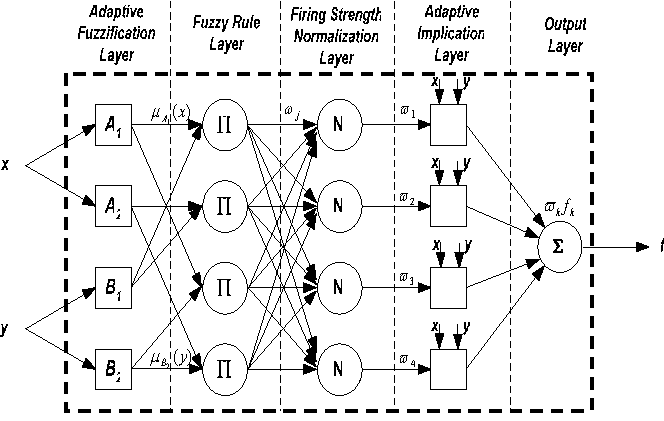
\includegraphics[width=.9\textwidth]{problematics/figure2}
    \caption{ANFIS architecture with two inputs, one outpur and four rules}
    \label{img:archit}
\end{figure}